\chapter{Result Discussion} \label{chap:results}
\begin{equation}
	\forall i \in N_\text{p}, \text{rho}_i (t_1) > \theta_\text{hard} \implies \forall t \in [t_1, t_1 + T_\text{reconnect}], F_i (t) = 0
\end{equation}

\begin{equation}
	\forall i \in N_\text{p}, t \in [t_1, t_1 + T_\text{soft}], \text{rho}_i (t) > \theta_\text{soft} \implies \forall t \in [t_1 + T_\text{soft}, t + T_\text{reconnect}], F_i (t)= 0
\end{equation}
In this chapter, the obtained results are thoroughly analysed and discussed. The performed experiments can be subdivided into 6 categories: Curtail Lower Limit (section \ref{sec:results-lower}), Limit Infeasible Curtailment Actions \ref{sec:results-limit}, Reward Tests \ref{sec:results-rewards}, \acp{GNN} Hyperparameter Tuning, \ac{GNN} Implementation Comparison \ref{sec:results-gnn-comp} and Scability Tests \ref{sec:results-scalability}.

\section{Implementation Details} \label{sec:results-implementation}

The development of \ac{GRL} algorithms posed as a complex and difficult problem. As mentioned in the literature review and restated in the problem statement, there is a scarse availability of open-source implementations and frameworks that are implemented to accommodate the implementation of these techniques. 

\subsection{Reproducibility}

A major concern and challenge brought with the technologies at hand was to implement a solution that brought reproducible results. This is critical to ensure appropriate analysis and calibration of the model as well as to allow other academics and interested readers to reproduce the results and follow the tuning process. \par

Initially, exploratory experiments with \textit{stable-baselines3} revealed that the \ac{DRL} algorithms were developed in a deterministic and reproducible nature but with the inclusion of the \textit{torch\_geometric}  \acp{GNN} the results were not consistent. \par

In this context, the documentation of both libraries were thoroughly analysed and studied and it was ensured that all of the appropriate seeds were being defined. However, results in the same machine still differed. This was later found to be related with the non-deterministic nature of some \textit{torch\_geometric} functions in the GPU, namely \textit{torch-scatter} operations \cite{NotReproducibleSetting} \cite{ReproducibilityPyTorchDocumentation}. \par

Although, at first, this issue seemed unsolvable, a specific parameter was found in the \textit{PyTorch} Documentation \cite{ReproducibilityPyTorchDocumentation} that successfully mitigated this problem and allowed for result reproducibility. Nevertheless, for different machines, the results still showed inconsistencies. \par

\begin{lstlisting}
	import torch
	torch.use_deterministic_algorithms(True)
\end{lstlisting}

\subsection{Flexibility}

One of the objectives that was also a large focus of the implemented solution, was to allow different combinations of \ac{DRL} and \ac{GNN} algorithms. Since \ac{GRL} still is a relatively recent field, it's important that research around this area builds foundations for other studies and this is facilitated with the developed flexible framework that enables experiments on other models that are currently unexplored. \par
With the advantages of having two popular frameworks for each type of algorithms with a consistent API for both made this goal easier to achieve than the former one associated with reproducibility. \par


\section{Reward Function} \label{sec:results-rewards}

Several implementations posed as relevant formulas to describe the reward function of the environment, namely three: Economic Reward, \acp{RES} Penalty Factor Reward and \acp{RES} Bonus Reward. The first considered only the saved cost in non-renewable generators operation, while the second and third accounted for \ac{RES} maximization in a penalty and bonus factor, respectively.
\par
Considering the new parameter introduced by both the Penalty and Bonus Factor rewards, $\beta$, the experiments took into account three distinct values: $\{0.4, 0.6, 0.8\}$.  \par
It's important to note that when evaluating and comparing reward functions, the average cumulative reward values retain different meanings. Furthermore, although still relevant to analyse the convergence of the models, other metrics were favoured, such as daily operating cost, abandoned \ac{RES} energy and the survival rate. \par

\begin{figure}[H]
	\centering
	\subfloat{}{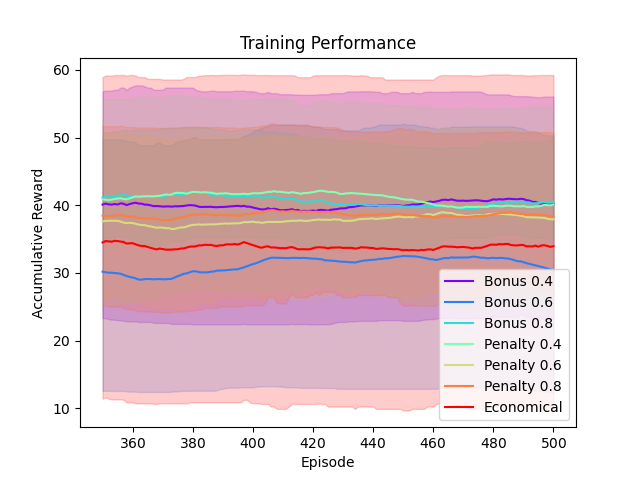
\includegraphics[width=.45\textwidth]{graphs/reward/training_performance.png}}
	\hskip1ex
	\subfloat{}{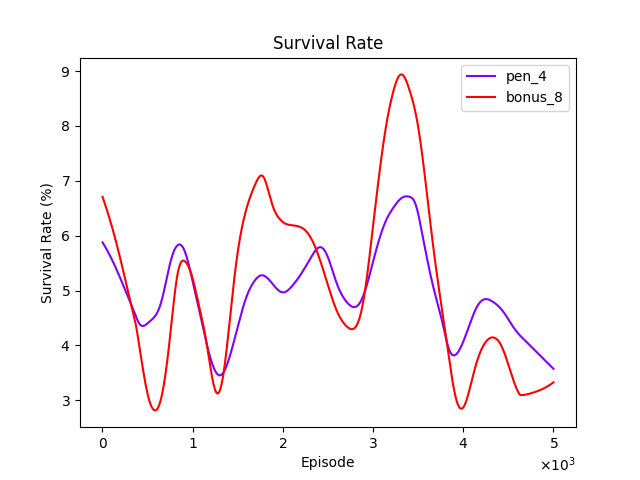
\includegraphics[width=.45\textwidth]{graphs/reward/survival_rate.png}} 
	\vfill
	\subfloat{}{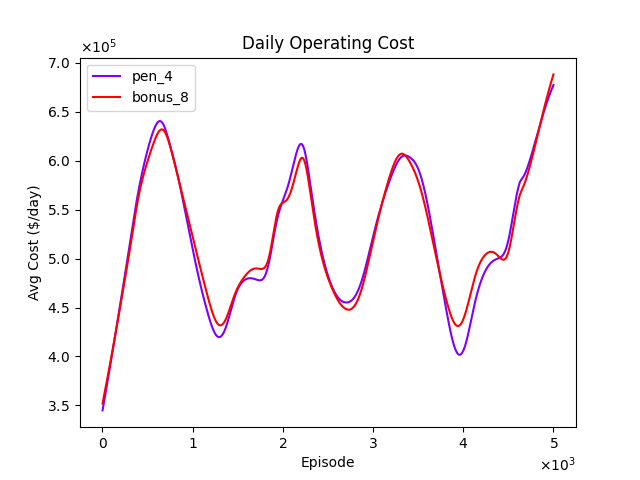
\includegraphics[width=.45\textwidth]{graphs/reward/daily_cost.png}} \hskip1ex
	\subfloat{}{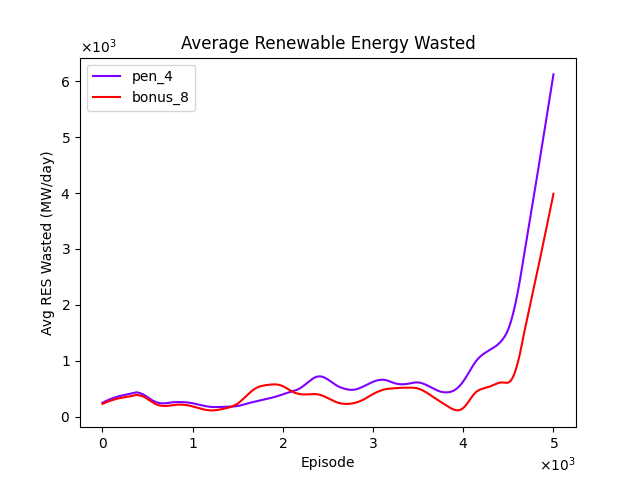
\includegraphics[width=.45\textwidth]{graphs/reward/res_wasted.png}} 
	\caption{Training Results of the Experiments concerning Observation Space.}
	\label{fig:train-reward}
\end{figure}

  \begin{table}[h!]
	\centering
	\caption{Test Results for Reward Parameters Experiments}
	\begin{tabular}{cccccc}
		\toprule
		\multirow{2}{*}{\textbf{reward}} & \multirow{2}{*}{\textbf{$\beta$}} & \multicolumn{4}{c}{\textbf{Metrics}} \\ 
		\cmidrule(lr){3-6}
		&  & \textbf{Avg. CR} & \textbf{Avg. Length} & \textbf{Avg. DOC} & \textbf{Avg. REW} \\ 
		\midrule
		bonus & 0.8 & 40.88 & 96.43 & 560927.60 & 3115.18 \\
		penalty & 0.4 & 40.57 & 80.75 & 565893.63 & 4100.20 \\
		bonus & 0.4 & 40.13 & 76.23 & 565757.16 & 3723.72  \\
		penalty & 0.8 & 38.22 & 76.35 & 555582.14 & 2612.34 \\
		penalty & 0.6 & 37.54 & 81.40 & 558362.82 & 2570.71 \\
		economical & - & 34.38 & 58.65 & 574981.17 & 2610.70 \\
		bonus & 0.6 & 30.78 & 55.06 & 566786.07 & 2750.34 \\
		% Add more rows as needed
		\bottomrule
	\end{tabular}
	\label{tab:test-reward}
\end{table}


\par
Results revealed that the proposed implementations were superior to the already defined Economic Reward both in survivability and overall performance of the models. The with the best results were observed in the Bonus Factor Reward with $\beta = 0.4$. Although





\begin{comment}
	* Best SAC and GNN parameters
	* Explain that SAC was used for most experiments as a baseline
\end{comment}

\section{Observation Space} \label{sec:results-obs}

Regarding the observation space, two matters were found to be worth to analyse. 
Firstly, it was hypothesized that using time keys (minute, hour, and day of the week) instead of the current step might help the model find temporal patterns in the sequential process that could yield performance improvements. \par
Additionally, given the complexity of the problem at hand, a min-max scale was applied in particular keys also with the goal of increasing learning efficency and overall performance. The scaling was applied to $P^\text{NRES}_i (t)$, $P^\text{RES}_i (t)$, and $\overline{P^\text{RES}_i} (t)$. \par

\begin{equation}
	x' = \frac{x - \min x}{\max x - \min x}
\end{equation}

  \begin{table}[h!]
	\centering
	\caption{Test Results for Observation Space Parameters Experiments}
	\begin{tabular}{cccccc}
		\toprule
		\multirow{2}{*}{\textbf{step}} & \multirow{2}{*}{\textbf{scaled}} & \multicolumn{4}{c}{\textbf{Metrics}} \\ 
		\cmidrule(lr){3-6}
		& & \textbf{Avg. CR} & \textbf{Avg. Length} & \textbf{Avg. DOC} & \textbf{Avg. REW} \\ 
		\midrule
		
		True & False & 40.00 & 65.26 & 559046.91 & 2302.77 \\
		False & False  & 56.31 & 85.65 & 565029.79 & 2088.03 \\
		True & True & 39.93 & 66.036 & 567707.16  & 2581.26 \\
		False & True & 45.33 & 69.96 & 552337.96 & 2520.84 \\
		% Add more rows as needed
		\bottomrule
	\end{tabular}
	\label{tab:test-obs}
\end{table}


\section{Action Space} \label{sec:results-action}

The initial exploratory experiments and posterior training performance analysis showed significant instability and lack of convergence of \ac{DRL} models. During the experimentation phase, the developed implementations, SAC and GCN-SAC, showed a significantly reduced survival rate. This posed a substantial problem since models failed to survive enough steps to appropriately learn economic policies, leading to relatively short results in their test phase. \par

\begin{table}[h!]
	\centering
	\caption{Test Results for \texttt{no\_curtail} Environment Parameter Search}
	\begin{tabular}{ccccc}
		\toprule
		\multirow{2}{*}{\textbf{no\_curtail}} & \multicolumn{4}{c}{\textbf{Metrics}} \\ 
		\cmidrule(lr){2-5}
		&  \textbf{Avg. CR} & \textbf{Avg. Length} & \textbf{Avg. DOC} & \textbf{Avg. REW} \\ 
		\midrule
		True & 130.15 & 676.74 & 536423.98 & 0.0 \\
		False & 22.13 & 37.14 & 619721.30  & 10315.47  \\
		% Add more rows as needed
		\bottomrule
	\end{tabular}
	\label{tab:test-curtail}
\end{table}

Upon further research, the root of this problem was found to be related to the inclusion of curtailment actions, which made the action space more complex and, in turn, severely affected the models' performance. Table \ref{tab:test-curtail} clearly states this problem, by highlighting the test results of two models with and without curtailment actions. As observed, the inclusion of curtailment actions caused an average cumulative reward decrease of 83.00\% in relation to the model without these type of actions. Additionally, the survivability of the worst model was also significantly inferior, with an average episode length of 37.14 steps. \par
It was found that during the exploratory phase, the abrupt changes in curtailment caused infeasible states of the system and, consequently, an early episode truncation. This caused the model to perform very poorly and, as a consequence, severely affected the learning efficiency, since the algorithms were not managing to survive enough steps to appropriately learn optimal dispatch policies. \par
With the purpose of further analysing and solving this problem, two methods described in the following subsections \ref{sec:results-limit} and \ref{sec:results-lower} were experimented to mitigate it.


\subsection{Limit Curtailment Infeasible States} \label{sec:results-limit}

The first method that was analysing the effect of using the grid2op  \texttt{LIMIT\_INFEASIBLE\_CURTAILMENT\_STORAGE\_ACTION} parameter, which according to its own long name and documentation limits infeasible system states derivative from curtailment (and storage) actions. \par
For this purpose, another model was trained with this flag set to \texttt{True}. 

\begin{comment}
	TODO -> LIMIT Experiements Graphs and tables
\end{comment}



The training results confirmed the initial suspicions, demonstrating that while performance is significantly and negatively affected when curtailment actions are included, by setting the \texttt{LIMIT\_INFEASIBLE\_CURTAILMENT\_STORAGE\_ACTION} the model was able to achieve higher results than without the parameter. As observed in table \ref{tab:test-limit}, the usage of the parameter translated into an improvement of 346.63 \% in average cumulative reward and 1100.02 \% in survival rate compared with the worst model. \par

\begin{figure}[H]
	\centering
	\subfloat{}{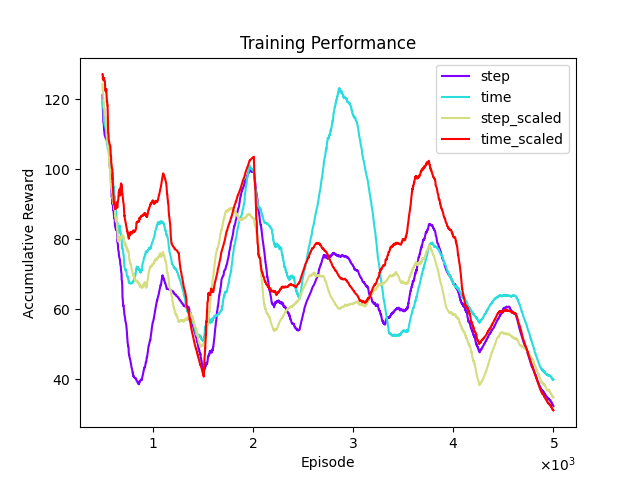
\includegraphics[width=.45\textwidth]{graphs/obs/training_performance.png}}
	\hskip1ex
	\subfloat{}{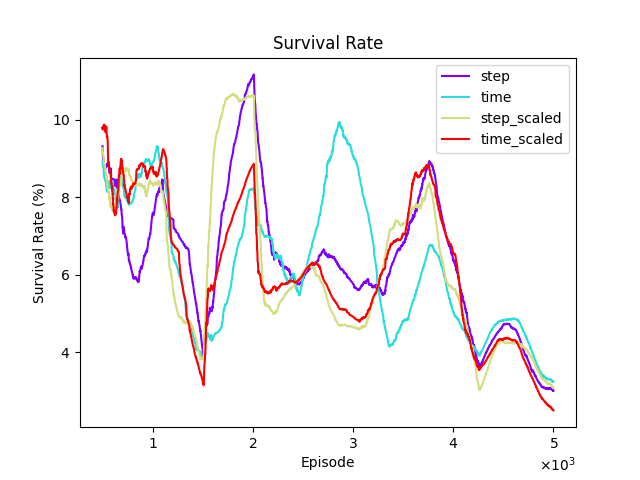
\includegraphics[width=.45\textwidth]{graphs/obs/survival_rate.png}} 
	\vfill
	\subfloat{}{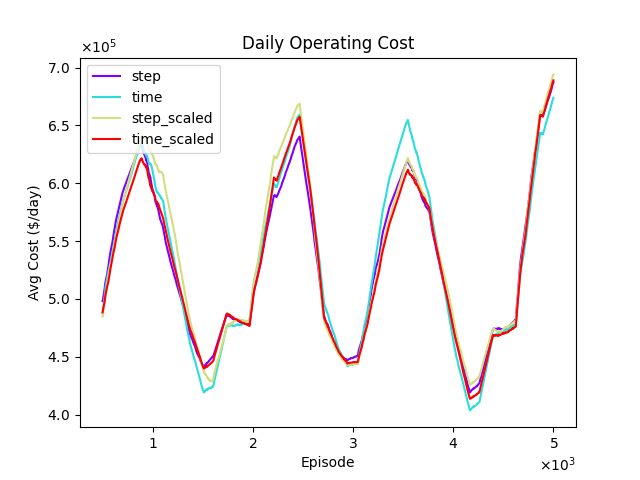
\includegraphics[width=.45\textwidth]{graphs/obs/daily_cost.png}} \hskip1ex
	\subfloat{}{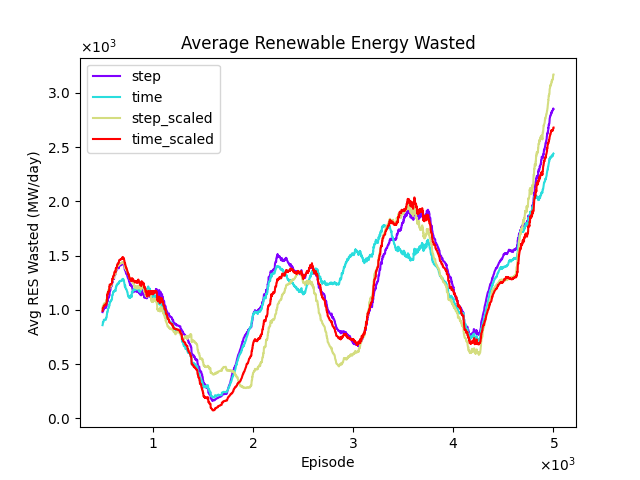
\includegraphics[width=.45\textwidth]{graphs/obs/res_wasted.png}} 
	\caption{Training Results of the Experiments concerning Observation Space.}
	\label{fig:train-obs}
\end{figure}

\begin{table}[h!]
	\centering
	\caption{Test Results for \texttt{limit\_inf} \textit{Grid2Op} Parameter Experiments}
	\begin{tabular}{cccccc}
		\toprule
		\multirow{2}{*}{\textbf{no\_curtail}} & \multirow{2}{*}{\textbf{limit\_inf}} & \multicolumn{4}{c}{\textbf{Metrics}} \\ 
		\cmidrule(lr){3-6}
		&  & \textbf{Avg. CR} & \textbf{Avg. Length} & \textbf{Avg. DOC} & \textbf{Avg. REW} \\ 
		\midrule
		True & False & 130.15 & 676.74 & 536423.98 & 0.00 \\
		False & True  & 98.84 & 445.77 & 588610.57 & 8039.41 \\
		False & False & 22.13 & 37.14 & 619721.30 & 10315.47 \\
		
		% Add more rows as needed
		\bottomrule
	\end{tabular}
	\label{tab:test-gcn-limit}
\end{table}

Although its usage has an apparent positive effect on model performance, it still did not mitigate the concerns related to the introduced complexity of curtailment actions. The model without these actions still outperformed the others by a large margin, outlining a difference of 31.31 reward units on average to the second-best model. The proposed method failed to mitigate the advantage brought by the behaviour of the model without curtailment actions, which by default uses all of the available renewable energy at each timestep, resulting in 0.0 MW of wasted \ac{RES} energy.

\subsection{Curtailment Lower Limit} \label{sec:results-lower}

Another possible solution to the problem of added intricacy advent from including curtailment actions is the definition of a lower bound for curtailment actions that restricts the model operation in this regard. \par

\begin{equation} \label{eq:linear-decay}
	y = 1 - \frac{(1 - \underline{P^\text{RES}}) E_\text{train}}{E_\text{decay\_end}}
\end{equation}

\begin{equation} \label{eq:sqrt-decay}
	y = (1 - \underline{P^\text{RES}}) \sqrt[\alpha]{\frac{E_\text{decay\_end} - E_\text{train}}{E_\text{train}}}
\end{equation}

Reflecting on the secondary goal of maximising the usage of generated renewable energy, the idealisation of a lower limit to confine the curtailment action space became a feasible solution to aid in the model's learning efficiency. In this manner, this condition was included in the implementation along with three possible strategies applied solely in the training stage:
\begin{itemize}
	\item Fixed lower bound
	\item Linear decreasing lower bound
	\item Square Root decreasing lower bound
\end{itemize}


An experiment compared the performance of the proposed strategies and the impact of this method on the former one introduced in subsection \ref{sec:results-limit}. The test results are observable in table \ref{tab:test-decay}.

\begin{table}[h!]
	\centering
	\caption{Test Results for \texttt{decay\_type} \ac{GCN} Parameter Experiments}
	\begin{tabular}{ccccc}
		\toprule
		  \multirow{2}{*}{\textbf{decay}} & \multicolumn{4}{c}{\textbf{Metrics}} \\ 
		\cmidrule(lr){2-5}
		& \textbf{Avg. CR} & \textbf{Avg. Length} & \textbf{Avg. DOC} & \textbf{Avg. REW} \\ 
		\midrule
		sqrt & 153.77 & 628.19 & 579978.88 & 7356.86 \\
		fixed & 122.58 & 461.28 & 541391.22 & 7480.09 \\
		linear & 111.52 & 289.36 & 550832.62 & 7092.56 \\
		None & 98.84 & 445.77 & 588610.57 & 8039.41 \\
		% Add more rows as needed
		\bottomrule
	\end{tabular}
	\label{tab:test-decay}
\end{table}

Results proved that the introduced curtailment lower bounds considerably increased the model's training performance and convergence, with the square root decay method achieving the overall highest average cumulative reward during the test phase. The models with a fixed lower bound and linear decay also exceeded the method presented in the former subsection without outperforming the model without curtailment. The best model outperformed the one without curtailment actions in average cumulative reward by 18.15 \%, which showed the relevance of including these actions to learning efficiency and justified their usage.\par
Nevertheless, the model with no curtailment reached a slightly higher survival rate without curtailment actions, as observable in table \ref{tab:test-curtail-comp}.


\begin{table}[h!]
	\centering
	\caption{Test Results for \texttt{decay\_type} \ac{GCN} Parameter Experiments}
	\begin{tabular}{ccccccc}
		\toprule
		\multirow{2}{*}{\textbf{no\_curtail}} & \multirow{2}{*}{\textbf{limit\_inf}} & \multirow{2}{*}{\textbf{decay}} & \multicolumn{4}{c}{\textbf{Metrics}} \\ 
		\cmidrule(lr){4-7}
		&  & & \textbf{Avg. CR} & \textbf{Avg. Length} & \textbf{Avg. DOC} & \textbf{Avg. REW} \\ 
		\midrule
		False & True & sqrt & 153.77 & 628.19 & 579978.88 & 7356.86 \\
		False & False & sqrt & 153.77 & 628.19 & 579978.88 & 7356.86 \\
		True & False & None & 130.15 & 676.74 & 536423.98 & 0.00 \\
		False & True & None & 98.84 & 445.77 & 588610.57 & 8039.41 \\
		False & False & None &  22.13 & 37.14 & 619721.30 & 10315.47 \\
		
		% Add more rows as needed
		\bottomrule
	\end{tabular}
	\label{tab:test-curtail-comp}
\end{table}


Interestingly, the combination of both proposed methods had no performance improvement, with the most significant being observed in the lower bound method. This clearly shows the superiority of this solution over the other, which, on its own, did not justify the usage of curtailment actions. However, given that the usage of the \texttt{LIMIT\_INFEASIBLE\_CURTAILMENT\_STORAGE\_ACTION} parameter also had a positive effect on performance and the author was not sure that the simultaneous usage of both methods always translated into the same learning efficiency as using only the lower bound method, a combination of both solutions was considered as the optimal procedure.

\section{\acp{GNN} Hyperparameter Tuning} \label{sec:results-gnn}

As a key area of this research work, the \ac{GNN} component of the proposed algorithm was given a special emphasis on what accounts for hyperparameter tuning. Concrete experiments were devised to assess the performance of different parameter combinations, mainly focusing on the \ac{GCN} architecture. This section is organised as follows: in this first subsection \ref{sec:results-aggr}, the performance of the several available aggregation schemes is unveiled and analysed; in subsection \ref{sec:results-layers} the focus is shifted towards the number of \ac{GNN} layers; in the following subsection \ref{sec:results-gcn-param} the effect of other specific \ac{GCN} parameters is analysed, and, lastly, in the last subsection \ref{sec:results-gat-param} the same process is performed for the \ac{GAT} architecture. \par 


\subsection{Aggregate Function} \label{sec:results-aggr}

The aggregation function is a crucial component of \ac{GNN} algorithms, and because of this fact, it was the first parameter investigated. An experiment was conducted to ascertain the best-performing aggregation function of the \ac{GCN} architecture, and the available schemes include the following:
\begin{itemize}
	\item \texttt{Sum}
	\item \texttt{Max}
	\item \texttt{Min}
	\item \texttt{Mean}
	\item \texttt{Mul}
\end{itemize}
\begin{equation}
	\max (\mathcal{X}) = \max_{x_i \in \mathcal{x}} x_i
\end{equation}


\begin{figure}[ht]
	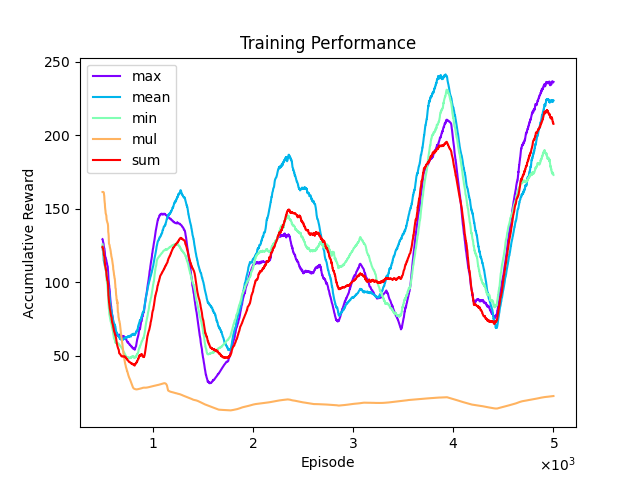
\includegraphics[width=0.75\textwidth]{graphs/aggr/training_performance.png}
	\caption{Training Performance per Aggregation Scheme}
	\label{fig:train-perf-aggr}
\end{figure}

As observed in figure \ref{fig:train-perf-aggr}, training performance  only revealed an apparently poor performing multiplication scheme, with other schemes achieving somewhat similar results. However, this aggregation function ended up achieving a significantly higher survival rate during training, which is verified in the test results depicted in table \ref{tab:test-aggr}. \par

\begin{figure}[ht]
	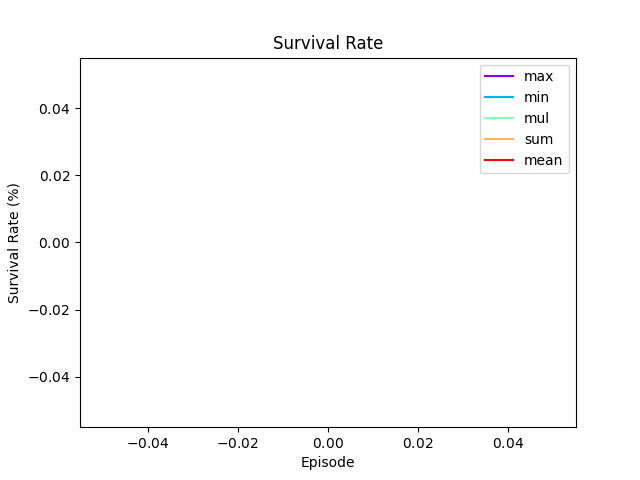
\includegraphics[width=0.75\textwidth]{graphs/aggr/survival_rate.png}
	\caption{Survival Rate per Aggregation Scheme}
	\label{fig:train-surv-aggr}
\end{figure}

As observed in figure \ref{fig:train-perf-aggr}, training performance revealed a poorly performing multiplication scheme compared to the other tested functions. However, the multiplication function yielded a significantly high average length of 1104.06 in tests, over 43\% of the model with the second-best survivability (sum), while at the same time achieving only 15.76 of average cumulative reward, which is a significantly lower value compared with the model with the second-to-last reward of 80.89. As observed in the test results, this case is primarily due to a high average daily operating cost, close to four thousand euros more than any other model. Beyond that, this model did not perform optimally when analysing the average energy from \ac{RES} wasted, with over three thousand megawatts of unused renewables in relation to every other model. \par

\begin{table}[h!]
	\centering
	\caption{Test Results for \texttt{aggr} \ac{GCN} Parameter Experiments}
	\begin{tabular}{ccccc}
		\toprule
		\multirow{2}{*}{\textbf{aggr}} & \multicolumn{4}{c}{\textbf{Metrics}} \\ 
		\cmidrule(lr){2-5}
		&  \textbf{Avg. CR} & \textbf{Avg. Length} & \textbf{Avg. DOC} & \textbf{Avg. REW} \\ 
		\midrule
		max & 119.16 & 677.75 & 560219.45 & 6564.49 \\
		sum & 114.58 & 768.58 & 569952.37 & 7268.28 \\
		mean & 92.90 &  551.24 & 557637.84 & 6268.06 \\
		min & 80.89 & 495.70 & 559033.63 & 6687.94 \\
		mul & 15.76 & 1104.06 & 608319.66 & 10305.96 \\
		% Add more rows as needed
		\bottomrule
	\end{tabular}
	\label{tab:test-gcn-aggr}
\end{table}


The test results also showed that the function with the best average cumulative reward was \texttt{max}, outperforming the second-placed \texttt{sum} by almost five reward points. Furthermore, this model managed to do better than average in most metrics while simultaneously being outperformed in all of them. This shows the balance between the importance of cost saving, the maximisation of renewable energy and model survivability that the algorithm must equate for optimally solving the problem of \ac{DED}. \par
In this manner, although the \textit{max} function yielded the best performance only by a small margin, the author still chose it as the optimal aggregation scheme.

\begin{comment}
	TODO ->>> TOTAL TIME
\end{comment}

\subsection{Layers} \label{sec:results-layers}

Another critical characteristic of \ac{GNN} architecture is the number of layers. Another separate experiment was devised to assess the optimal value for this parameter, considering the \texttt{max} aggregation scheme, which, as exposed in the last subsection \ref{sec:results-aggr}, yielded the best results. The models had one to six \ac{GCN} layers, and the results are observable in table \ref{tab:test-layers}.

\begin{figure}[H]
	\centering
	\subfloat{}{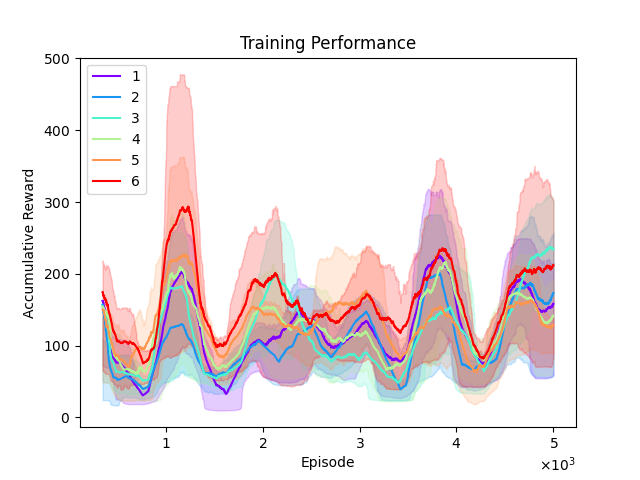
\includegraphics[width=.45\textwidth]{graphs/layers/training_performance.png}}
	\hskip1ex
	\subfloat{}{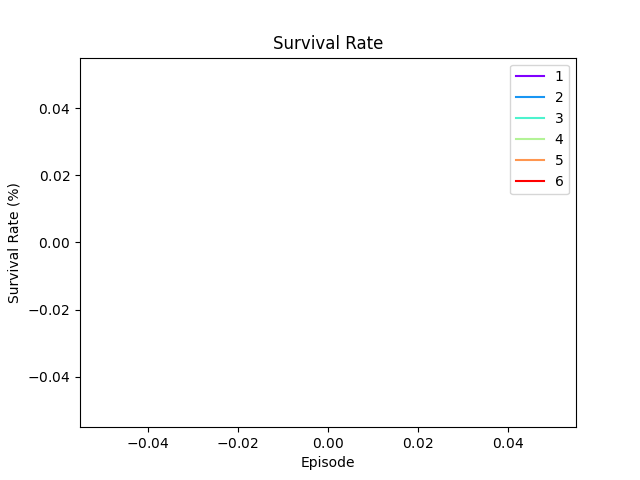
\includegraphics[width=.45\textwidth]{graphs/layers/survival_rate.png}} 
	\vfill
	\subfloat{}{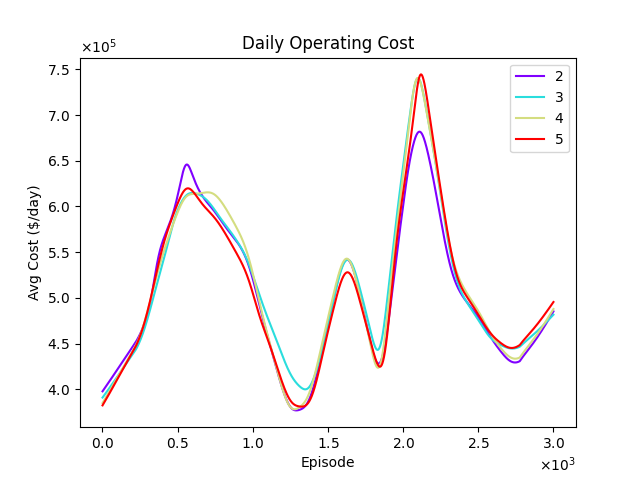
\includegraphics[width=.45\textwidth]{graphs/layers/daily_cost.png}} \hskip1ex
	\subfloat{}{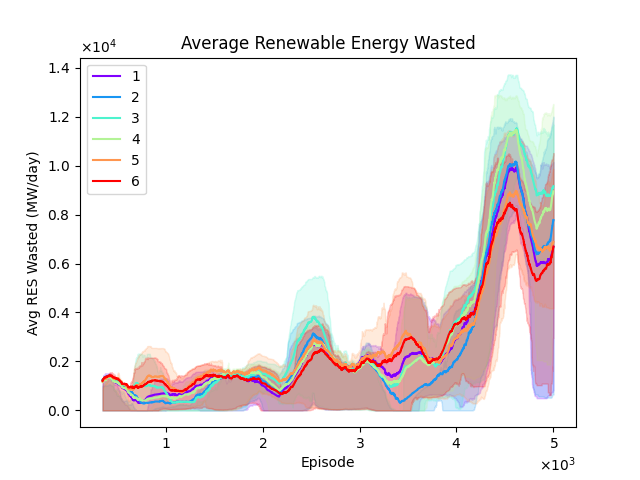
\includegraphics[width=.45\textwidth]{graphs/layers/res_wasted.png}} 
	\caption{Training Results of models with 1, 2, 3, 4, 5, and 6 \ac{GNN} Layers}
	\label{fig:train-layers}
\end{figure}

Regarding the study conducted around this \ac{GNN} characteristic, a configuration of six layers stands out from the rest, reaching an average cumulative reward of 135.75 reward units. This value represents a 13.92\% improvement regarding the second-best model in this metric, which was the one-layer network.

  \begin{table}[h!]
	\centering
	\caption{Test Results for \texttt{num\_layers} \ac{GCN} Parameter Experiments}
	\begin{tabular}{ccccc}
		\toprule
		\multirow{2}{*}{\textbf{num\_layers}} & \multicolumn{4}{c}{\textbf{Metrics}} \\ 
		\cmidrule(lr){2-5}
		&  \textbf{Avg. CR} & \textbf{Avg. Length} & \textbf{Avg. DOC} & \textbf{Avg. REW} \\ 
		\midrule
		
		6 & 135.75 & 487.09 & 560147.77 & 5862.49 \\
		1 & 119.16 & 677.75 & 560219.45 & 6564.49 \\
		3 & 110.73 & 736.32 & 567510.58 & 7116.24 \\
		4 & 98.67 & 451.51 & 577464.90 & 8641.05 \\
		5 & 92.97 & 286.65 & 550205.21 & 6397.41 \\
		2 & 91.58 & 694.67 & 575093.64 & 5989.95 \\
		% Add more rows as needed
		\bottomrule
	\end{tabular}
	\label{tab:test-layers}
\end{table}

Generally, the calibration process has failed to reach ideal levels of survivability.
Once again, the top-performing model in cumulative performance did not correspond to the best metric, the three-layered network, with an average survival rate of 36.52\%. This value corresponds to an average survivability of 2.56 days per weekly episode, which, in a real-world scenario, models would break the power grid constraints after only a few days of operation. 

\subsection{Output Features} \label{sec:results-out}
 
  \begin{table}[h!]
	\centering
	\caption{Test Results for \texttt{out\_channels} \ac{GCN} Parameter Experiments}
	\begin{tabular}{ccccc}
		\toprule
		\multirow{2}{*}{\textbf{out\_channels}} & \multicolumn{4}{c}{\textbf{Metrics}} \\ 
		\cmidrule(lr){2-5}
		&  \textbf{Avg. CR} & \textbf{Avg. Length} & \textbf{Avg. DOC} & \textbf{Avg. REW} \\ 
		\midrule
		3 & & & & \\
		6 & & & & \\
		18 & & & & \\
		36 & & & & \\
		% Add more rows as needed
		\bottomrule
	\end{tabular}
	\label{tab:test-gcn-out}
\end{table}

\subsection{\ac{GCN} Parameters} \label{sec:results-gcn-param}

Some particular \ac{GNN} parameters not covered in the last subsections were also deemed relevant to analyse. This examination was motivated by an exploratory investigation that revealed the potential performance increase of using these parameters. \par
The \texttt{act\_first} parameter controls if the \ac{GNN} activation function, which is ReLU, is applied before the computation of the symmetric normalisation coefficients. The other parameter analysed was the \texttt{improved} flag, which defines whether the model computes $mathbf{\hat{A}}$ as $\mathbf{A} + 2\mathbf{I}$. \par
In this context, a grid search was conducted around these two parameters, whose test results are observable in table \ref{tab:test-gcn-params}.
 
 \begin{figure}[H]
 	\centering
 	\subfloat{}{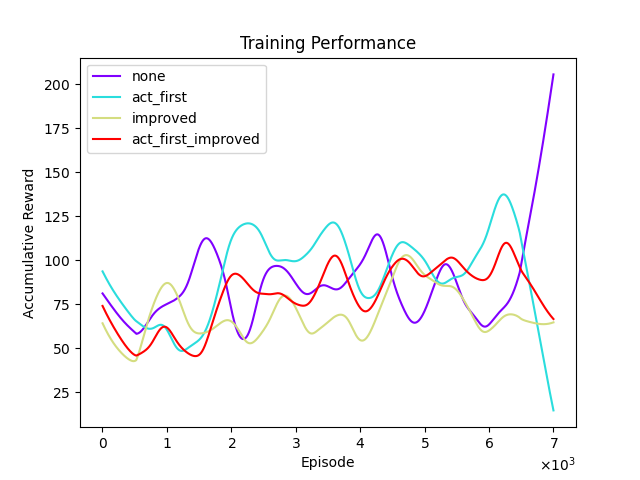
\includegraphics[width=.45\textwidth]{graphs/gnn_param/training_performance.png}}
 	\hskip1ex
 	\subfloat{}{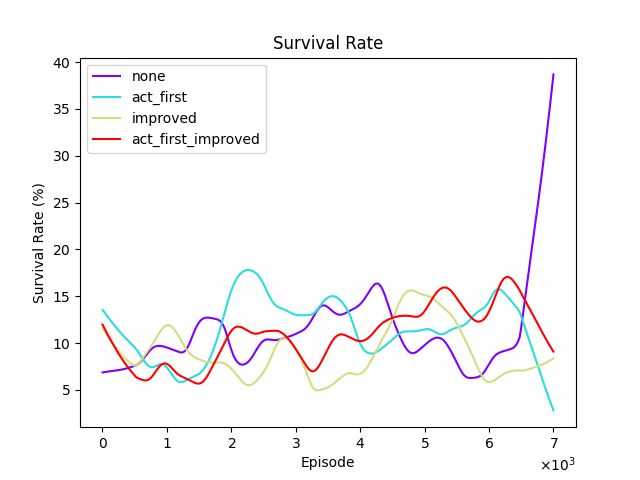
\includegraphics[width=.45\textwidth]{graphs/gnn_param/survival_rate.png}} 
 	\vfill
 	\subfloat{}{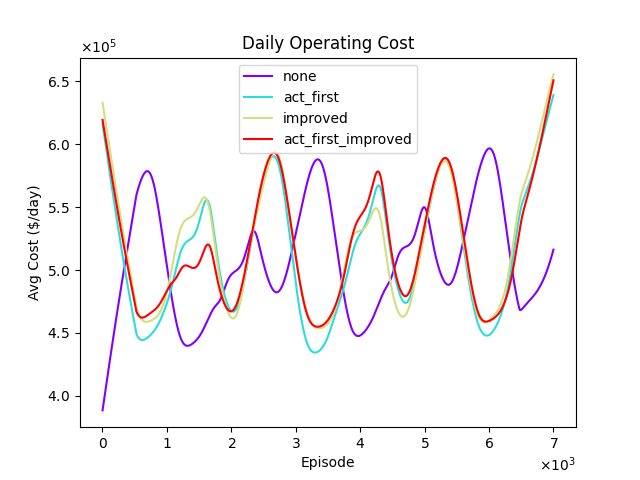
\includegraphics[width=.45\textwidth]{graphs/gnn_param/daily_cost.png}} \hskip1ex
 	\subfloat{}{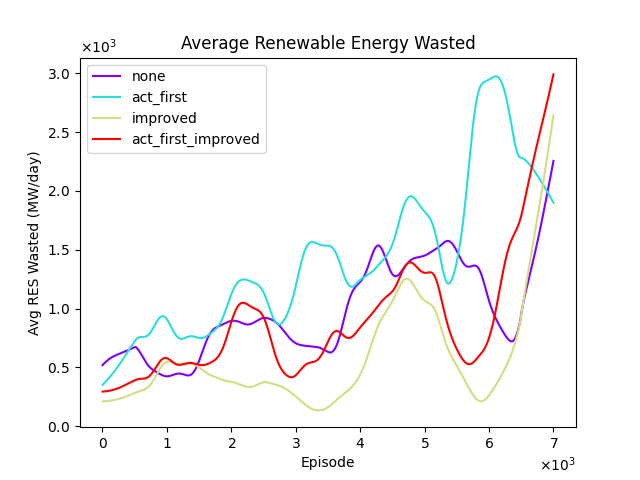
\includegraphics[width=.45\textwidth]{graphs/gnn_param/res_wasted.png}} 
 	\caption{Training Results of models with 2, 3, 4 and 5 \ac{GNN} Layers}
 	\label{fig:train-gcn-param}
 
 \end{figure}
 
 
 
  \begin{table}[h!]
 	\centering
 	\caption{Test Results for \texttt{act\_first} and \texttt{improved} \ac{GCN} Parameter Search}
 	\begin{tabular}{cccccc}
 		\toprule
 		\multirow{2}{*}{\textbf{act\_first}} & \multirow{2}{*}{\textbf{improved}} & \multicolumn{4}{c}{\textbf{Metrics}} \\ 
 		\cmidrule(lr){3-6}
 		&  &  \textbf{Avg. CR} & \textbf{Avg. Length} & \textbf{Avg. DOC} & \textbf{Avg. REW} \\ 
 		\midrule
 		True & False & 118.97 & 640.40 & 564201.23 & 7167.22 \\
 		True & True & 101.26 & 738.60 & 546592.78 & 6297.46 \\
 		False & False & 78.62 & 759.82 & 575798.57& 7640.76 \\
 		False & True & 75.29 & 328.78 & 548378.53 & 5043.04 \\
 		% Add more rows as needed
 		\bottomrule
 	\end{tabular}
 	\label{tab:test-gcn-params}
 \end{table}
 
 
 The use of \texttt{act\_first} positively affected performance, considering the two best results. In contrast, the models that performed the activation after normalisation failed to surpass 100 reward units. Furthermore, the models benefited from not defining \texttt{improved}, translating into a cumulative reward improvement in both cases. In this manner, the chosen optimal configurations for these parameters were \texttt{act\_first = True} and \texttt{improved = False}, corresponding to the combination used for the best-performing model.
 
\subsection{\ac{GAT} Parameters} \label{sec:results-gat-param}
 
As another prominent state-of-the-art architecture, the \ac{GAT} network was also target to some tuning in specific parameters. This seemed appropriate given the tuning process the \ac{GCN} network was particularly subject to, intending to also leverage the specific attributes of the \ac{GAT} architecture. The optimal combination of \texttt{aggr}, \texttt{num\_layers}, and \texttt{out\_channels} observable for the \ac{GCN} model was reused in this architecture. While this was not an optimal approach, this decision was taken given the timing constraints of the project and the often significant amount of training time. \par

In this manner, an experiment was conducted around the three most relevant parameters of this model: \texttt{act\_first}, \texttt{heads} and \texttt{v2}. The first, as seen in the previous subsection, positively affected the model's test results and learning efficiency, which encouraged further analysis. \par

The second and third parameters are specific to the \ac{GAT} network, with the first representing the number of attention heads used in the model and the second consisting of a flag that controls the use of the GATv2 architecture proposed in \cite{brodyHowAttentiveAre2022}. \par

This study used a random search of these parameters to ascertain the optimal combination, training 10 models for 3000 episodes each using the \textit{Ray Tune} library. The models were trained for 1, 2, and 3 heads and the test results are observable in the table \ref{tab:tune-gat}. \par


\begin{table}[h!]
	\centering
	\caption{Test Results for the \texttt{act\_first}, \texttt{heads} and \texttt{v2} \ac{GAT} Parameter Search}
	\begin{tabular}{ccccccc}
		\toprule
		\multirow{2}{*}{\textbf{act\_first}} & \multirow{2}{*}{\textbf{heads}} & \multirow{2}{*}{\textbf{v2}} & \multicolumn{4}{c}{\textbf{Metrics}} \\ 
		\cmidrule(lr){4-7}
		&  &  & \textbf{Avg. CR} & \textbf{Avg. Length} & \textbf{Avg. DOC} & \textbf{Avg. REW} \\ 
		\midrule
		% Example row, repeat this for each combination of act_first, heads, and v2
		True  & 3 & True  & 117.09 & 258.93 & 582144.59 & 7216.87 \\ 
		%True  & 3 & True  & 116.15 & 530.90 & 574232.74 & 8371.55 \\ 
		False & 3 & False & 111.41 & 726.20 & 569354.23 & 7403.57 \\ 
		True  & 1 & True  & 94.46  & 594.57 & 571177.15 & 6785.37 \\ 
		True  & 2 & True  & 92.50  & 650.37 & 562035.66 & 7349.15 \\ 
		False & 3 & True  & 91.18  & 197.57 & 552279.16 & 8988.24 \\ 
		%True  & 2 & True  & 89.71  & 189.68 & 559698.91 & 9183.43 \\ 
		True  & 2 & False & 88.77  & 611.40 & 565936.09 & 7250.76 \\ 
		True  & 3 & False & 80.03  & 579.84 & 556860.38 & 6723.43 \\ 
		%True  & 2 & False & 79.79  & 618.38 & 552375.15 & 6020.04 \\ 
		True  & 1 & False & 76.94  & 522.30 & 574402.26 & 8366.63 \\ 
		False & 1 & False & 76.06  & 476.15 & 549382.92 & 7971.11 \\ 
		%False & 1 & False & 75.47  & 404.99 & 554022.72 & 6131.49 \\ 
		%True  & 3 & False & 75.35  & 316.04 & 578969.32 & 5335.20 \\ 
		%True  & 1 & False & 72.00  & 493.83 & 543896.22 & 4590.01 \\ 
		%True  & 1 & True  & 70.57  & 405.59 & 568212.03 & 7496.51 \\ 
		False & 1 & True  & 59.17  & 273.63 & 574194.39 & 5665.66 \\ 
		%False & 1 & True  & 51.67  & 209.71 & 553394.87 & 7579.73 \\ 
		\bottomrule
	\end{tabular}
	\label{tab:tune-gat}
\end{table}

Furthermore, the outcomes of the test phase revealed that the model with the best average cumulative reward was the one with \texttt{act\_first} and \texttt{heads} set and three \texttt{heads} with 117.09 reward units. However, this model showed a significantly low survival rate. In contrast, the best-performing model in survival rate, which was also the second-best model in cumulative reward, had the two parameters unset and three \texttt{heads} as well, which directed the choice of attention heads to this value.

With regards to using the second version of the \ac{GAT} architecture, the results show that out of the top five models in cumulative reward, four use GATv2 implementation. The test results displayed that this choice almost consistently outperformed the other. \par

Lastly, the \texttt{act\_first} parameter also showed acceptable performance, with three models in the top five best-performing and the being present best model. This conclusion closes the optimal combination of these parameters considered in the following comparison and scalability experiments.

\section{GNN Implementation Comparison} \label{sec:results-gnn-comp}

\begin{table}[h!]
	\centering
	\caption{Test Results for 36-bus Scenario}
	\begin{tabular}{ccccccc}
		\toprule
		\multirow{2}{*}{\textbf{Model}} & \multicolumn{6}{c}{\textbf{Metrics}} \\ 
		\cmidrule(lr){2-7}
		&  \textbf{Avg. CR} & \textbf{Avg. Length} & \textbf{Avg. DOC} & \textbf{Avg. REW} & \textbf{Avg. ST} & \textbf{TT} \\ 
		\midrule
		SAC & 342.84 & 1118.24 & 601896.45 & 5443.65 & 0.0029 & 47.76 \\
		GCN-SAC & 153.77 & 628.19 & 579978.88 & 7356.86 & 0.0097 & 31.11 \\
		GAT-SAC &105.75 & 231.88 & 564739.25 & 7070.78 & 0.0071 & 12.52 \\
		% Add more rows as needed
		\bottomrule
	\end{tabular}
	\label{tab:test-gnn}
\end{table}

\section{Scalability Tests} \label{sec:results-scalability}

\begin{table}[h!]
	\centering
	\caption{Test Results for the 118-bus Scenario}
	\begin{tabular}{lcccccc}
		\toprule
		\multirow{2}{*}{\textbf{Model}} & \multicolumn{6}{c}{\textbf{Metrics}} \\ 
		\cmidrule(lr){2-7}
		&  \textbf{Avg. CR} & \textbf{Avg. Length} & \textbf{Avg. DOC} & \textbf{Avg. REW} & \textbf{Avg. ST} & \textbf{TT} \\ 
		\midrule
		SAC & 81.98 & 361.92 & 2788763.38 & 4740.03 & 0.0067 & 14.82 \\
		GCN-SAC & 67.85 & 389.82 & 2901439.28 & 5323.58 & 0.0096 & 13.67 \\
		GAT-SAC & 54.31 & 240.28 & 2591733.60 & 4709.37 & 0.012 & 11.39 \\
		% Add more rows as needed
		\bottomrule
	\end{tabular}
	\label{tab:test-118}
\end{table}